\documentclass[a4paper,11pt]{paper}

\usepackage[T1]{fontenc}
\usepackage[spanish]{babel} 
\usepackage[utf8]{inputenc}
\usepackage{graphicx}
\usepackage{xcolor}
\usepackage{pdflscape}
\usepackage[breaklinks=true]{hyperref}


\renewcommand\familydefault{\sfdefault}
\usepackage{tgheros}
\usepackage[defaultmono]{droidmono}

\usepackage{amsmath,amssymb,amsthm,textcomp}
\usepackage{enumerate}
\usepackage{multicol}
\usepackage{tikz}
\usepackage{courier}

\usepackage{geometry}
\geometry{total={210mm,297mm},
left=25mm,right=25mm,%
bindingoffset=0mm, top=20mm,bottom=20mm}


\linespread{1.3}

\newcommand{\linia}{\rule{\linewidth}{0.5pt}}

% my own titles
\makeatletter
\renewcommand{\maketitle}{
\begin{center}
\vspace{2ex}
{\huge \textsc{\@title}}
\vspace{1ex}
\\
\linia\\
\@author \hfill \@date
\vspace{4ex}
\end{center}
}
\makeatother
%%%

% custom footers and headers
\usepackage{fancyhdr}
\pagestyle{fancy}
\lhead{}
\chead{}
\rhead{}
\lfoot{}
\cfoot{}
\rfoot{\thepage}
\renewcommand{\headrulewidth}{0pt}
\renewcommand{\footrulewidth}{0pt}
%

% code listing settings
\usepackage{listings}

\lstset{%
  language = Octave,
  backgroundcolor=\color{white},   
  basicstyle=\footnotesize\ttfamily,       
  breakatwhitespace=false,         
  breaklines=true,                 
  captionpos=b,                   
  commentstyle=\color{gray},    
  deletekeywords={...},           
  escapeinside={\%*}{*)},          
  extendedchars=true,              
  frame=single,                    
  keepspaces=true,                 
  keywordstyle=\color{green},       
  morekeywords={*,...},            
  numbers=left,                    
  numbersep=5pt,                   
  numberstyle=\footnotesize\color{gray}, 
  rulecolor=\color{black},         
  rulesepcolor=\color{blue},
  showspaces=false,                
  showstringspaces=false,          
  showtabs=false,                  
  stepnumber=1,                    
  stringstyle=\color{orange},    
  tabsize=2,                       
  title=\lstname,
  emphstyle=\bfseries\color{blue}%  style for emph={} 
} 

%% language specific settings:
\lstdefinestyle{Arduino}{%
    language = Octave,
    keywords={void, int boolean},%                 define keywords
    morecomment=[l]{//},%             treat // as comments
    morecomment=[s]{/*}{*/},%         define /* ... */ comments
    emph={HIGH, OUTPUT, LOW}%        keywords to emphasize
}

%% language specific settings:
\lstdefinestyle{Sql}{%
    language = Sql,
    keywords={MONEY,TINYINT,NVARCHAR,VARCHAR,int, bit,isnull,DATETIME,IDENTITY,XML,output,@@ROWCOUNT},%                 define keywords
    morecomment=[l]{--},%             treat -- as comments
    morecomment=[s]{/*}{*/},%         define /* ... */ comments
    emph={USE, GO, SET, ON, CREATE, TABLE, PRIMARY, INSERT, INTO, VALUES, AS, BEGIN, ALTER, SELECT, FROM,WHERE,END,PROCEDURE,DECLARE,AND,OR,UPDATE,IF,ELSE,MERGE,MATCHED,USING,WHEN,NOCOUNT,THEN,OUT}%        keywords to emphasize
}


%%%----------%%%----------%%%----------%%%----------%%%

\begin{document}


\title{Migración de palanca Showroom a Microservicios con MongoDB}

\author{César Gastón Cárdenas Códova}

\date{22/07/2018}
\pagenumbering{gobble}
\maketitle
\vspace*{\fill}
\begin{figure}[!h]
\centering
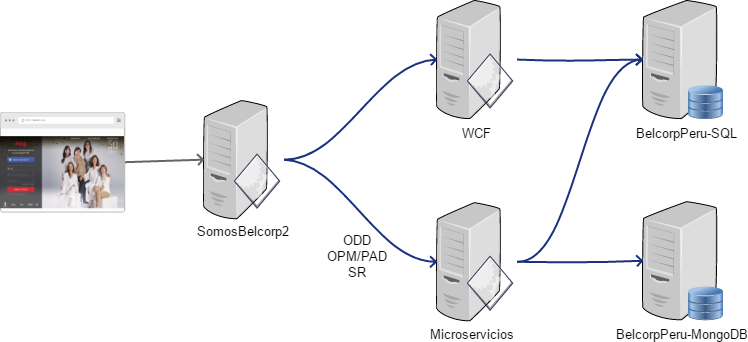
\includegraphics[width=0.9\textwidth]{imgs/arquitectura.png}
\end{figure}
\vspace*{\fill}

\newpage
\tableofcontents
\newpage
\phantomsection
 \listoffigures
\newpage
\pagenumbering{arabic}
\section{Administrador de contenido}

%%%----------%%%----------ESTRATEGIAS----------%%%----------%%%
\subsection{Gestión de estrategias}

\subsubsection{Nuevo Masivo}
\begin{figure}[h]
\centering
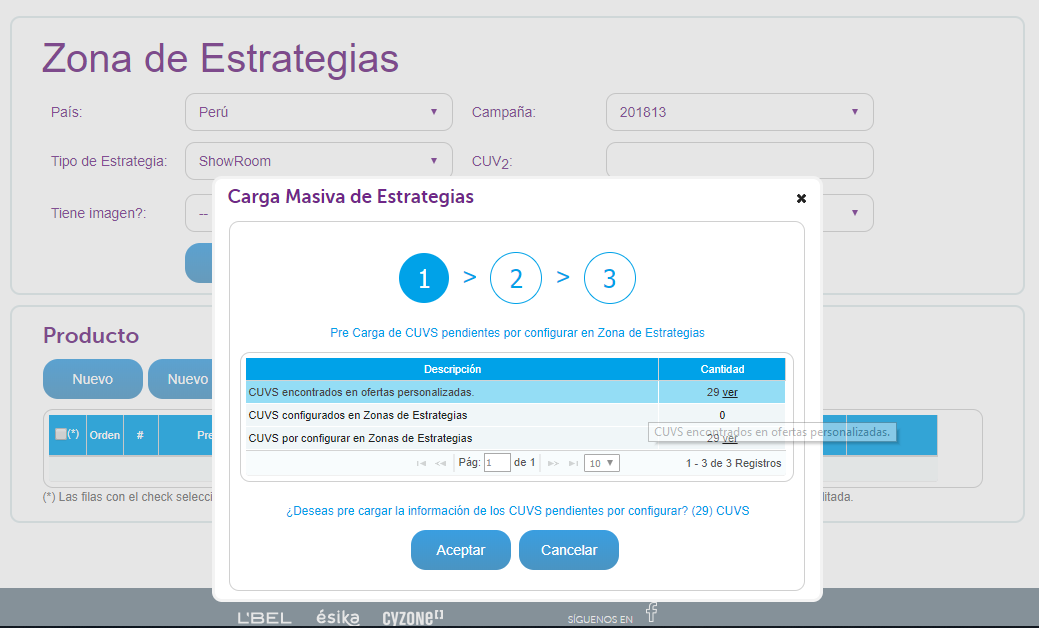
\includegraphics[width=1.0\textwidth]{imgs/Estrategia/FormularioNuevoMasivo.png}
\caption{Formulario nuevo masivo paso 1}
\end{figure}

\begin{figure}[h]
\centering
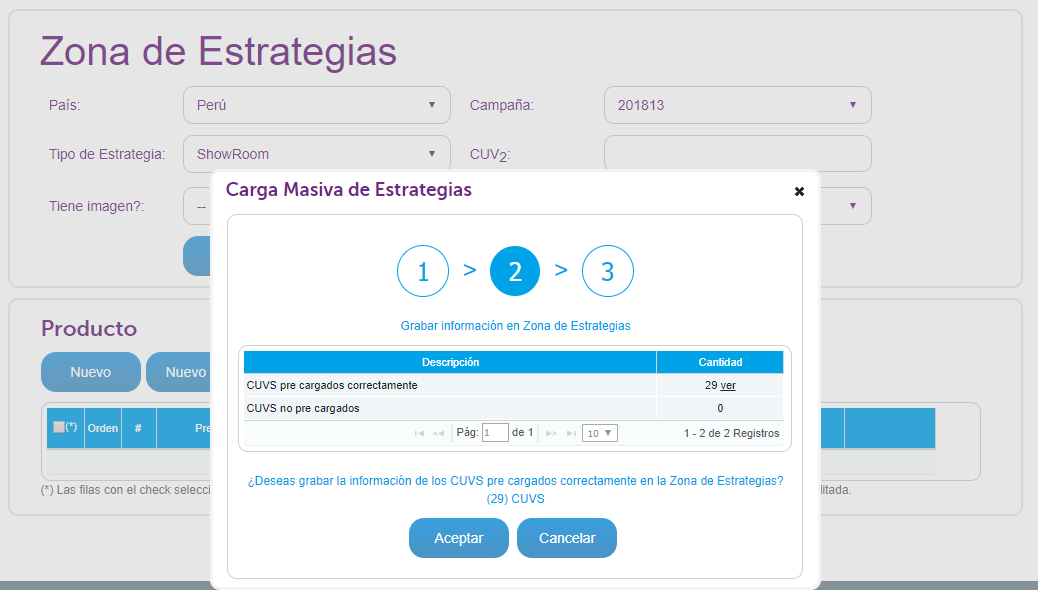
\includegraphics[width=1.0\textwidth]{imgs/Estrategia/FormularioNuevoMasivo2.png}
\caption{Formulario nuevo masivo paso 2}
\end{figure}

\begin{figure}[h]
\centering
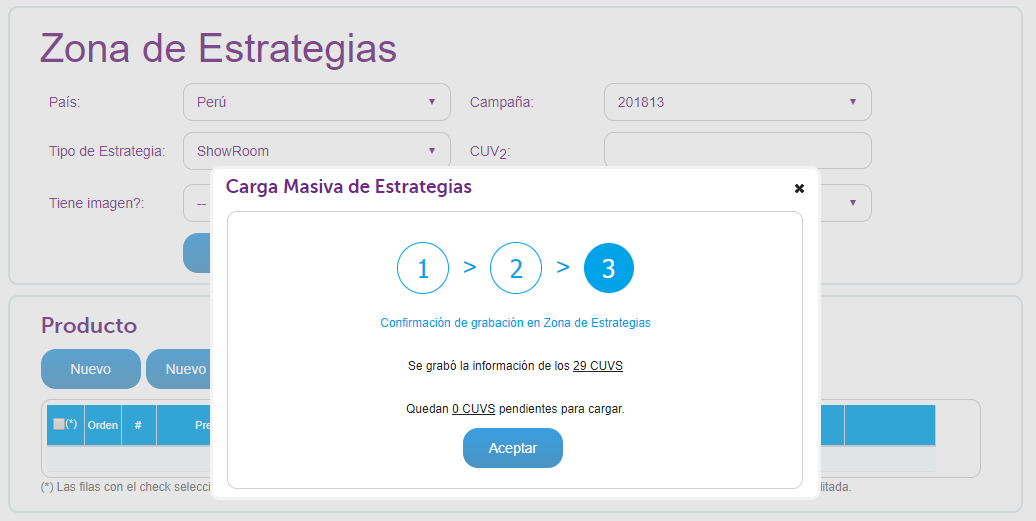
\includegraphics[width=1.0\textwidth]{imgs/Estrategia/FormularioNuevoMasivo3.png}
\caption{Formulario nuevo masivo paso 3}
\end{figure}

\newpage
\begin{landscape}
\begin{figure}[!h]
\centering
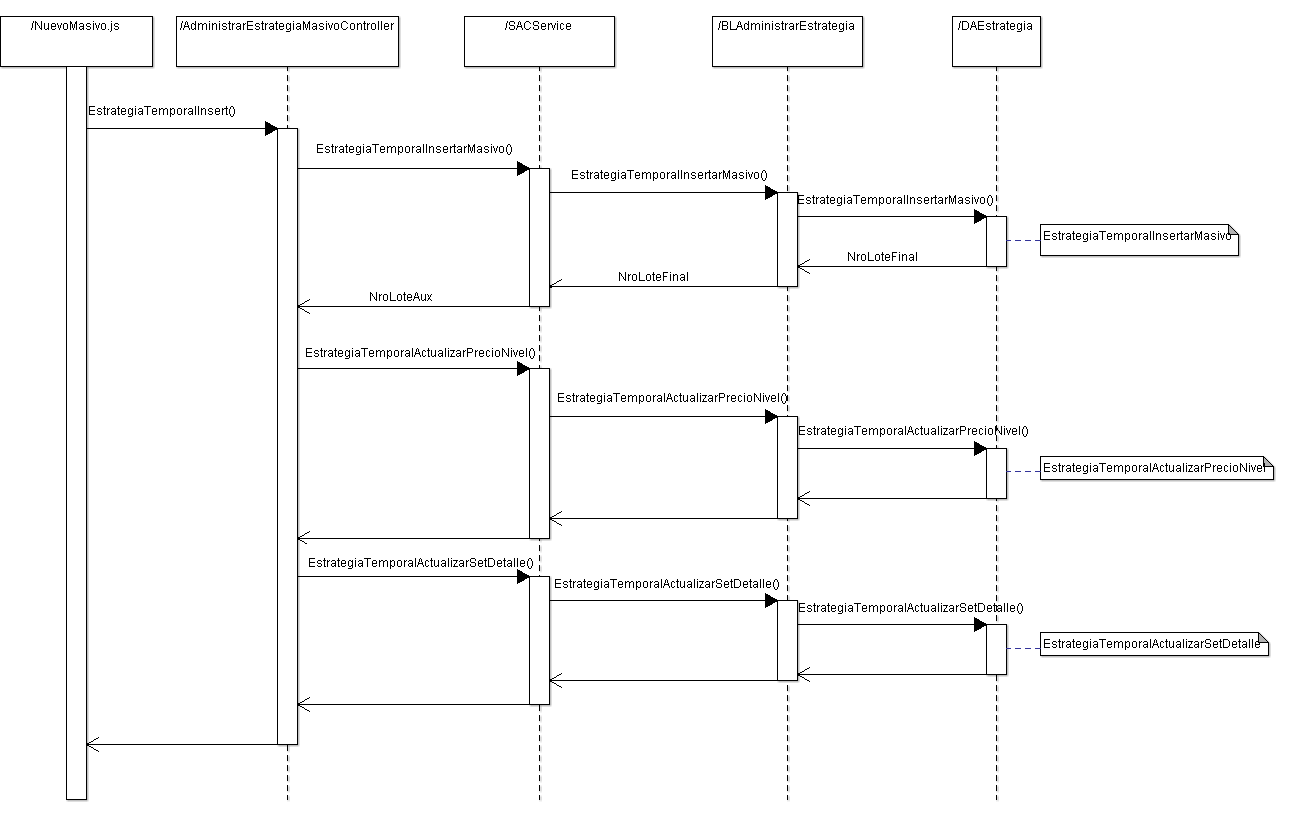
\includegraphics[width=1.5\textwidth]{imgs/Estrategia/NuevoMasivoTemporal.png}
\caption{Diagrama de secuencia Nuevo Masivo Temporal}
\end{figure}

\newpage
\begin{figure}[!h]
\centering
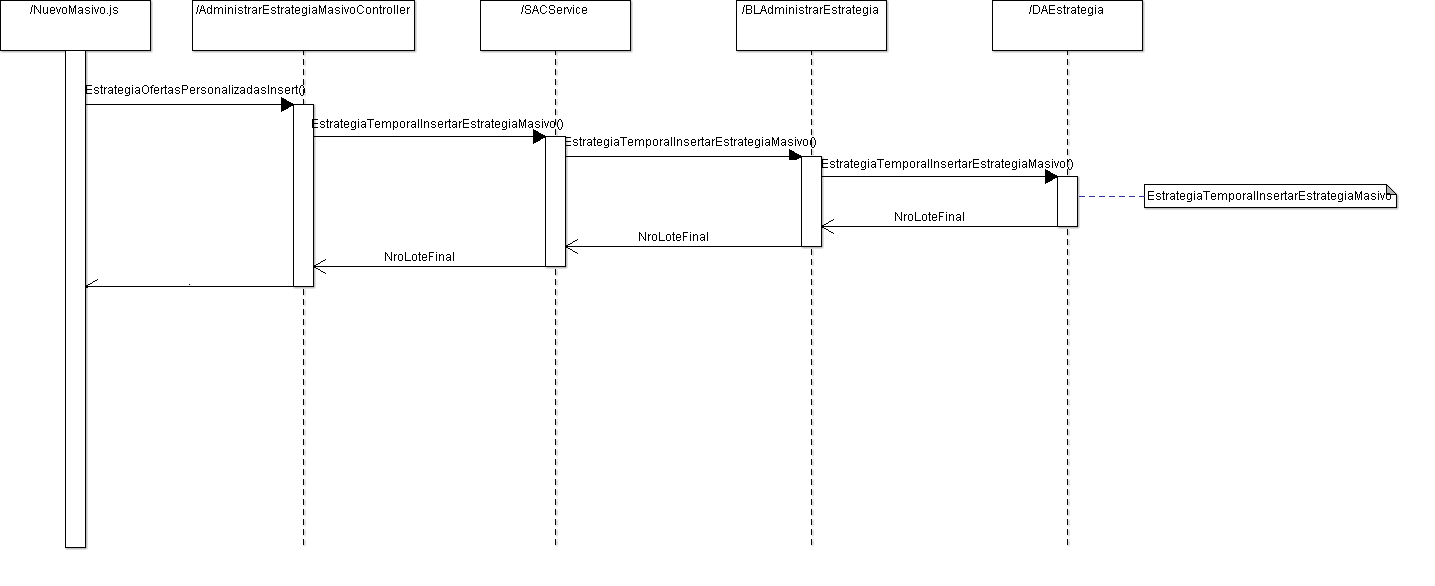
\includegraphics[width=1.5\textwidth]{imgs/Estrategia/NuevoMasivo.png}
\caption{Diagrama de secuencia Nuevo Masivo}
\end{figure}
\end{landscape} 

\lstinputlisting[style=Sql]{EstrategiaTemporalInsertarMasivo.sql}
\lstinputlisting[style=Sql]{EstrategiaTemporalActualizarPrecioNivel.sql}
\lstinputlisting[style=Sql]{EstrategiaTemporalActualizarSetDetalle.sql}
\lstinputlisting[style=Sql]{EstrategiaTemporalInsertarEstrategiaMasivo.sql}

\newpage
\subsubsection{Registrar/Editar Estrategia}
\begin{figure}[h]
\centering
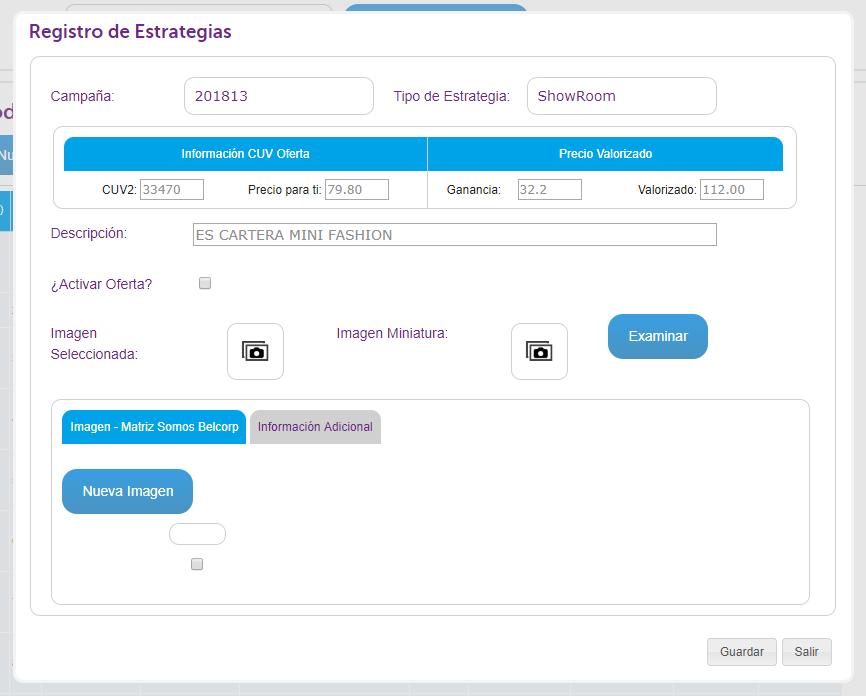
\includegraphics[width=1.0\textwidth]{imgs/Estrategia/RegistrarEstrategiaFormulario.png}
\caption{Formulario registro de estrategia}
\end{figure}

\newpage
\begin{landscape}
\begin{figure}[!h]
\centering
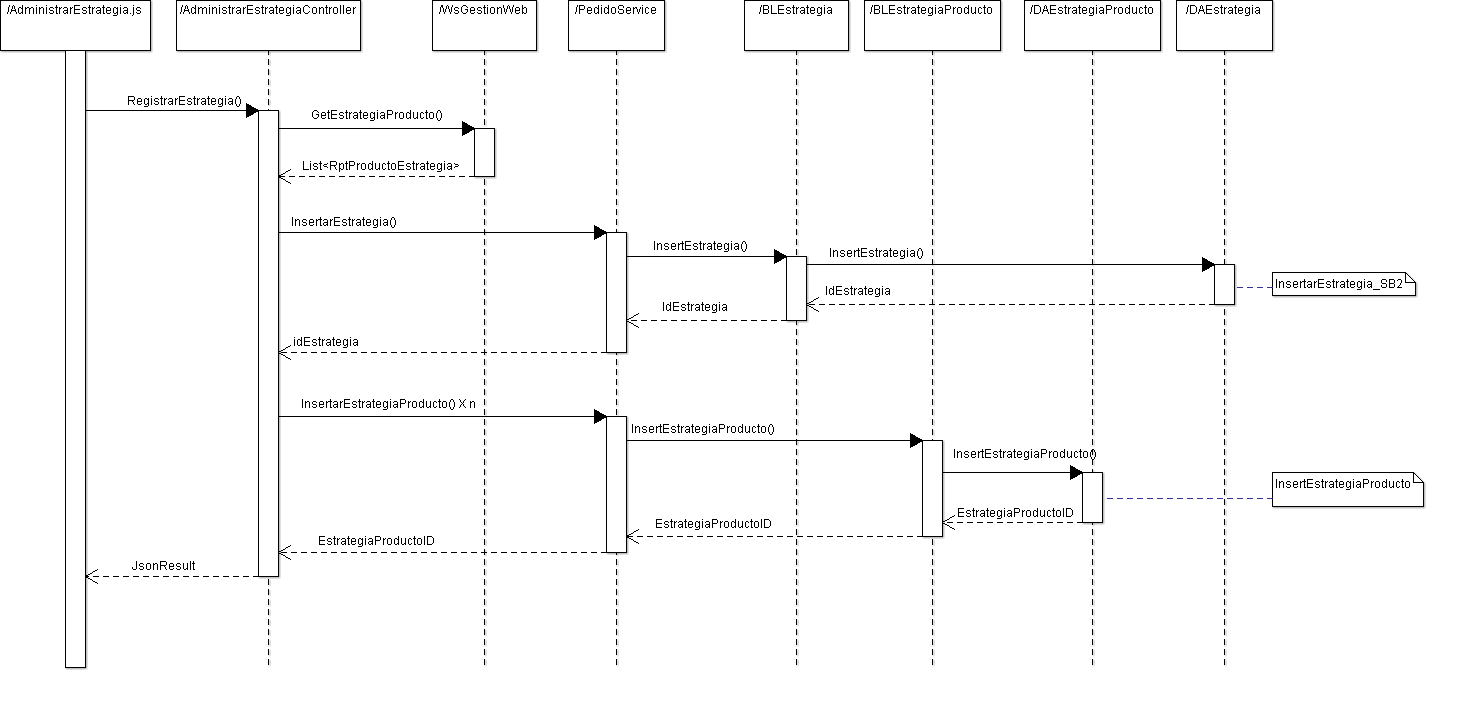
\includegraphics[width=1.5\textwidth]{imgs/Estrategia/RegistrarEstrategia.png}
\caption{Diagrama de secuencia Registrar/Editar Estrategia}
\end{figure}
\end{landscape} 
\lstinputlisting[style=Sql]{InsertarEstrategia_SB2.sql}
\lstinputlisting[style=Sql]{InsertEstrategiaProducto.sql}

\newpage
\subsubsection{Actualizar Descripción Masiva}
\begin{figure}[h]
\centering
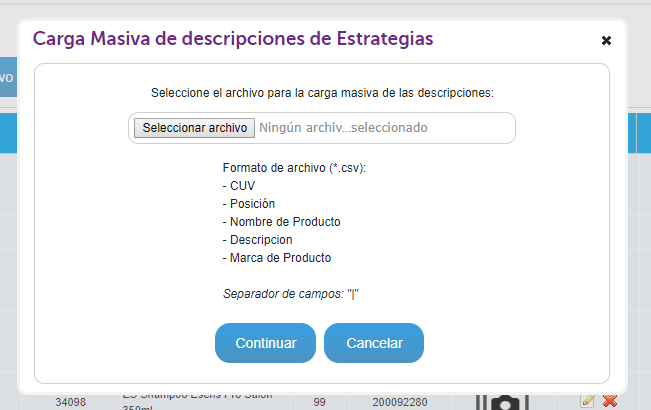
\includegraphics[width=1.0\textwidth]{imgs/Estrategia/FormularioActualizarDescripcionMasivaEstrategia.png}
\caption{Formulario registro de estrategia}
\end{figure}

\newpage
\begin{landscape}
\begin{figure}[!h]
\centering
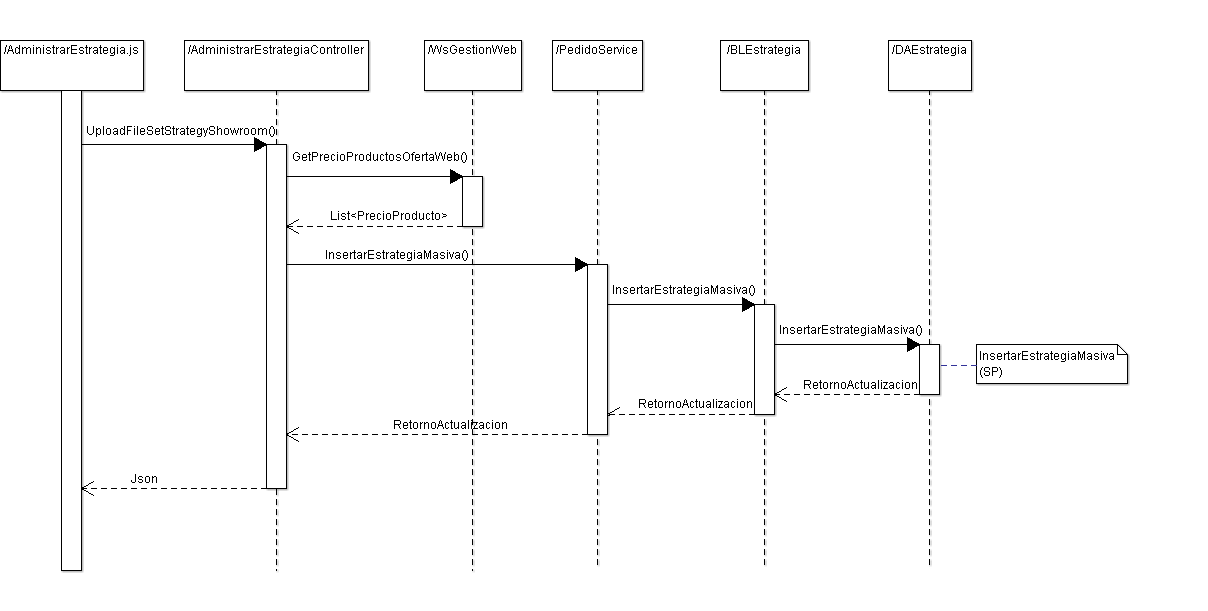
\includegraphics[width=1.5\textwidth]{imgs/Estrategia/ActualizarDescripcionMasivaEstrategia.png}
\caption{Diagrama de secuencia Actualizar descripción masiva}
\end{figure}
\end{landscape} 
\lstinputlisting[style=Sql]{InsertarEstrategiaMasiva.sql}

\newpage
\subsubsection{Activar/Desactivar estrategia}
\begin{figure}[h]
\centering
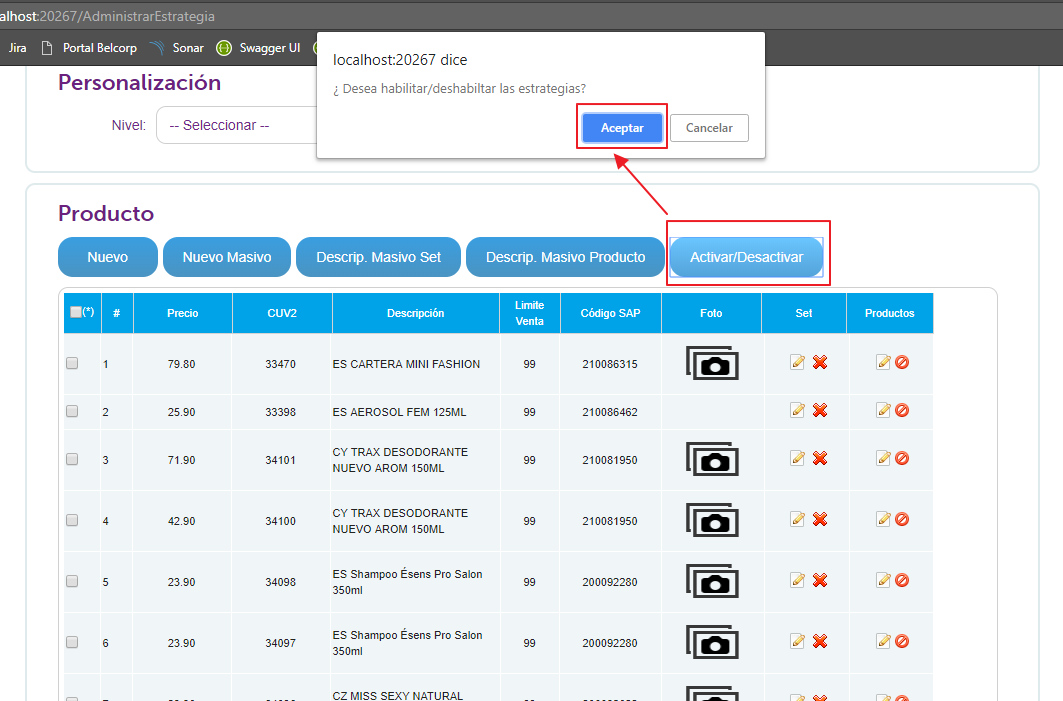
\includegraphics[width=1.0\textwidth]{imgs/Estrategia/FormularioActivarDesactivarEstrategia.png}
\caption{Formulario Activar/desactivar estrategia}
\end{figure}

\newpage
\begin{landscape}
\begin{figure}[!h]
\centering
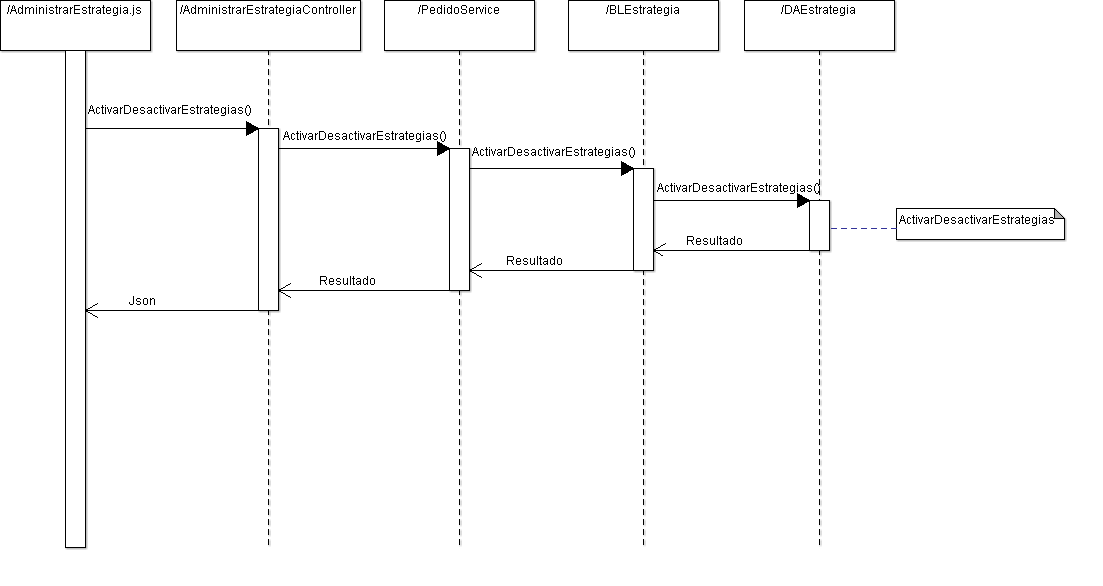
\includegraphics[width=1.5\textwidth]{imgs/Estrategia/ActivarDesactivarEstrategia.png}
\caption{Diagrama de secuencia Activar/desactivar estrategia}
\end{figure}
\end{landscape} 
\lstinputlisting[style=Sql]{ActivarDesactivarEstrategias.sql}

\newpage
\subsubsection{Deshabilitar Estrategia}
\begin{figure}[h]
\centering
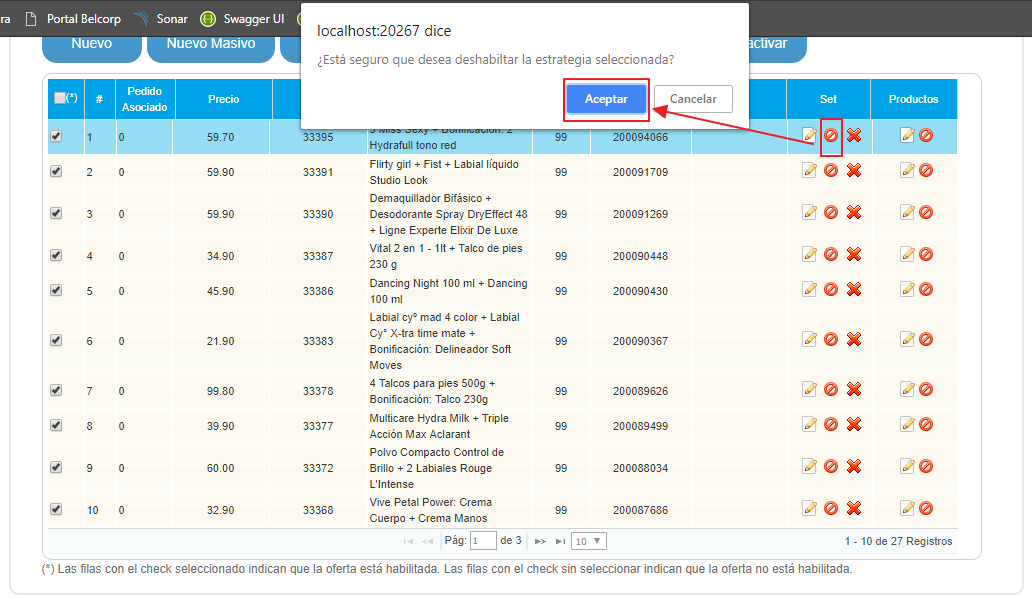
\includegraphics[width=1.0\textwidth]{imgs/Estrategia/FormularioDeshabilitar.png}
\caption{Formulario Deshabilitar estrategia}
\end{figure}

\newpage
\begin{landscape}
\begin{figure}[!h]
\centering
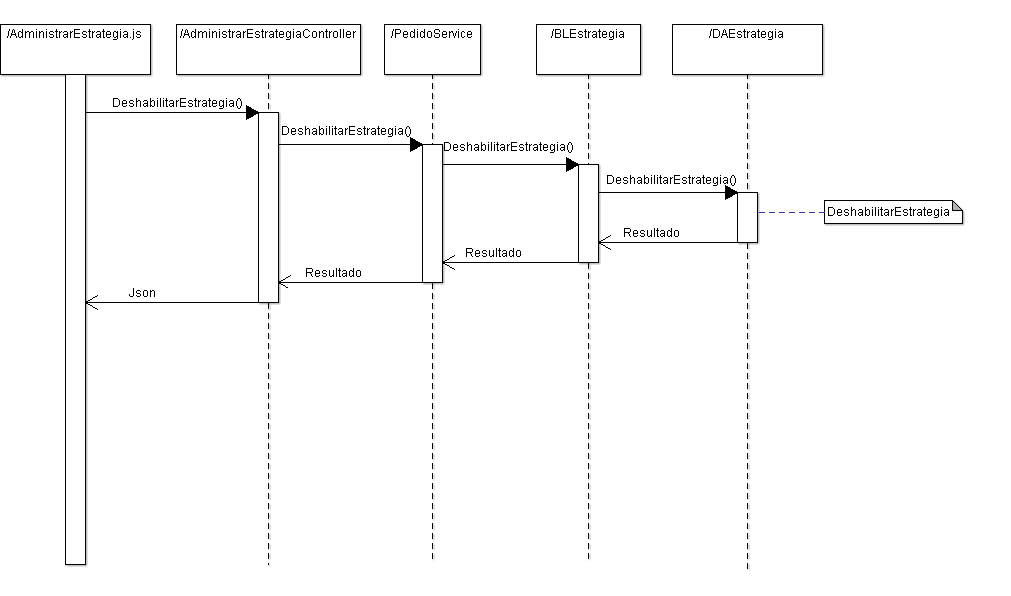
\includegraphics[width=1.5\textwidth]{imgs/Estrategia/Deshabilitar.png}
\caption{Diagrama de secuencia Deshabilitar estrategia}
\end{figure}
\end{landscape} 
\lstinputlisting[style=Sql]{DeshabilitarEstrategia.sql}

\newpage
\subsubsection{Eliminar Estrategia}
\begin{figure}[h]
\centering
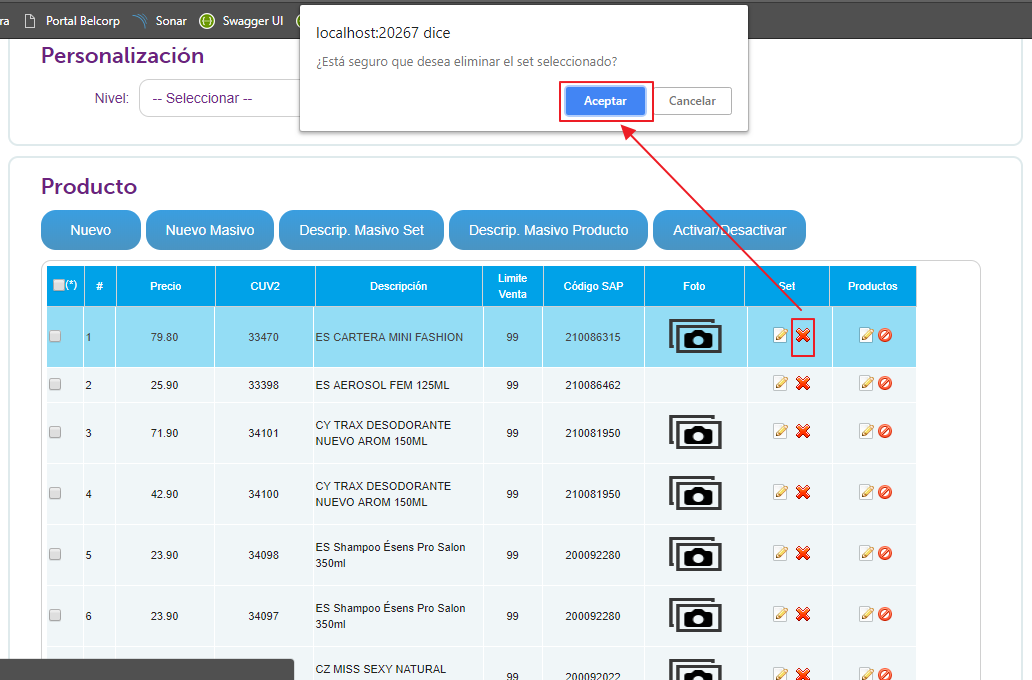
\includegraphics[width=1.0\textwidth]{imgs/Estrategia/FormularioEliminarEstrategia.png}
\caption{Formulario Eliminar estrategia}
\end{figure}

\newpage
\begin{landscape}
\begin{figure}[!h]
\centering
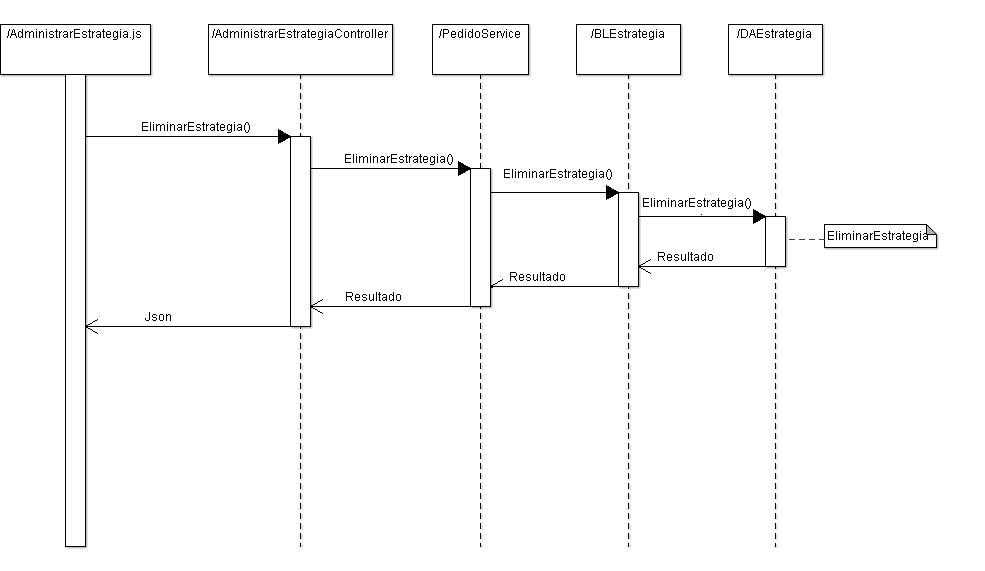
\includegraphics[width=1.5\textwidth]{imgs/Estrategia/EliminarEstrategia.png}
\caption{Diagrama de secuencia Actualizar descripción masiva}
\end{figure}
\end{landscape} 
\lstinputlisting[style=Sql]{EliminarEstrategia.sql}

%%%----------%%%----------EVENTOS----------%%%----------%%%
\newpage
\subsection{Gestión de eventos}

\begin{figure}[h]
\centering
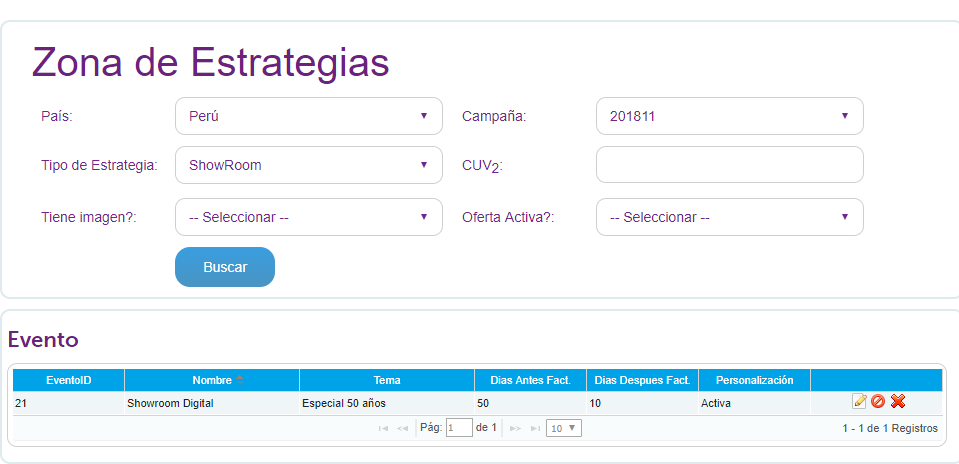
\includegraphics[width=1.0\textwidth]{imgs/Eventos/FormularioGestionEvento.png}
\caption{Formulario para administrar eventos}
\end{figure}

\newpage
\subsubsection{Modelo relacional}
\begin{figure}[h]
\centering
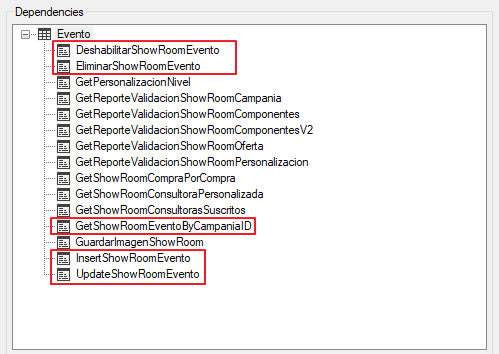
\includegraphics[width=1\textwidth]{imgs/Eventos/SPsAdm.png}
\caption{Procedimientos almacenados administrador de contenido}
\end{figure}

\newpage
\begin{figure}[h]
\centering
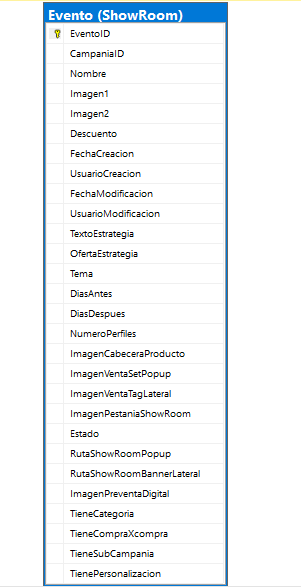
\includegraphics[width=0.5\textwidth]{imgs/Eventos/Tabla.png}
\caption{Tabla Evento}
\end{figure}

\newpage
\begin{figure}[h]
\centering
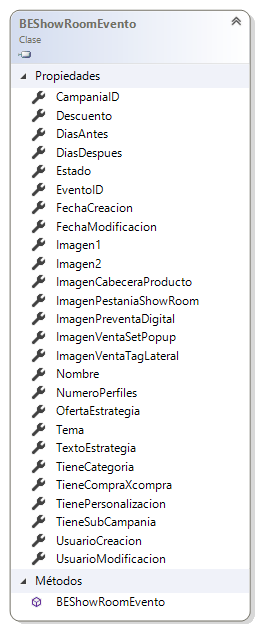
\includegraphics[width=0.4\textwidth]{imgs/Eventos/ClaseEvento.png}
\caption{Entidad Evento}
\end{figure}

\newpage
\begin{landscape}
\subsubsection{Consultar Evento}
\begin{figure}[!h]
\centering
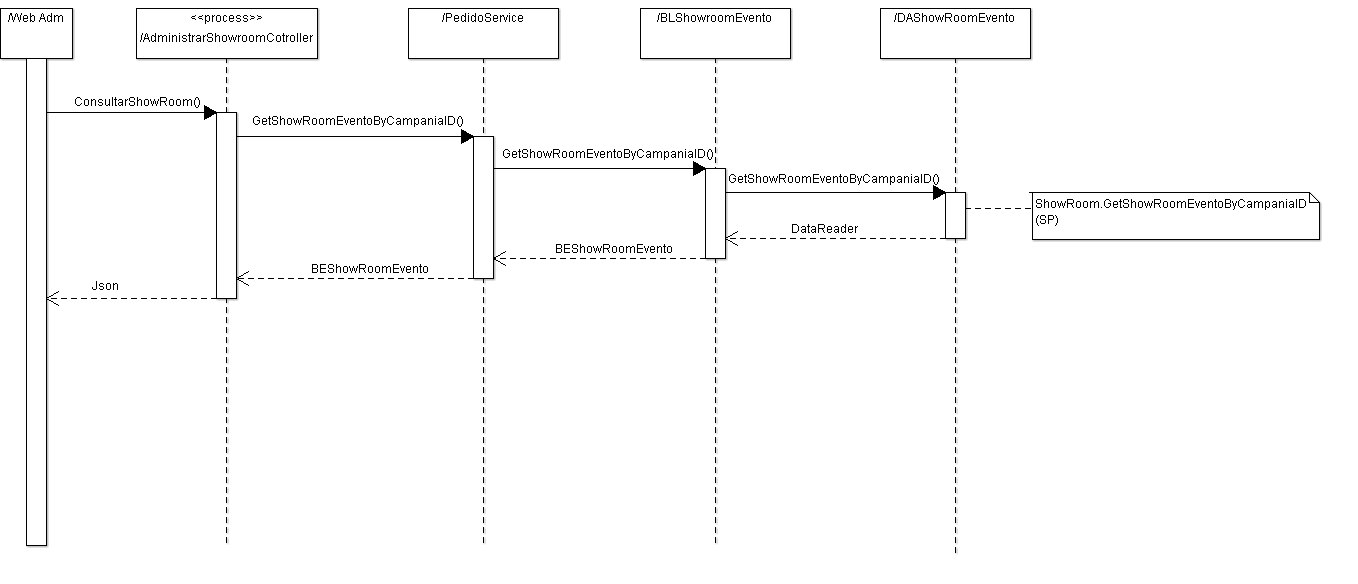
\includegraphics[width=1.5\textwidth]{imgs/Eventos/ConsultarEvento.png}
\caption{Diagrama de secuencia Consulta de Evento}
\end{figure}
\end{landscape} 


\lstinputlisting[style=Sql]{GetShowRoomEventoByCampaniaID.sql}


\newpage
\subsubsection{Crear Evento}

\begin{figure}[h]
\centering
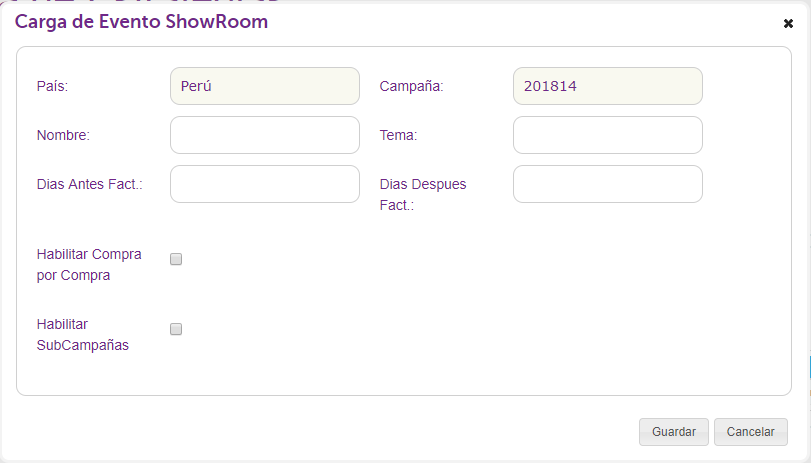
\includegraphics[width=1.0\textwidth]{imgs/Eventos/FormularioNuevoEvento.png}
\caption{Formulario para administrar eventos}
\end{figure}

\begin{landscape}
\begin{figure}[!h]
\centering
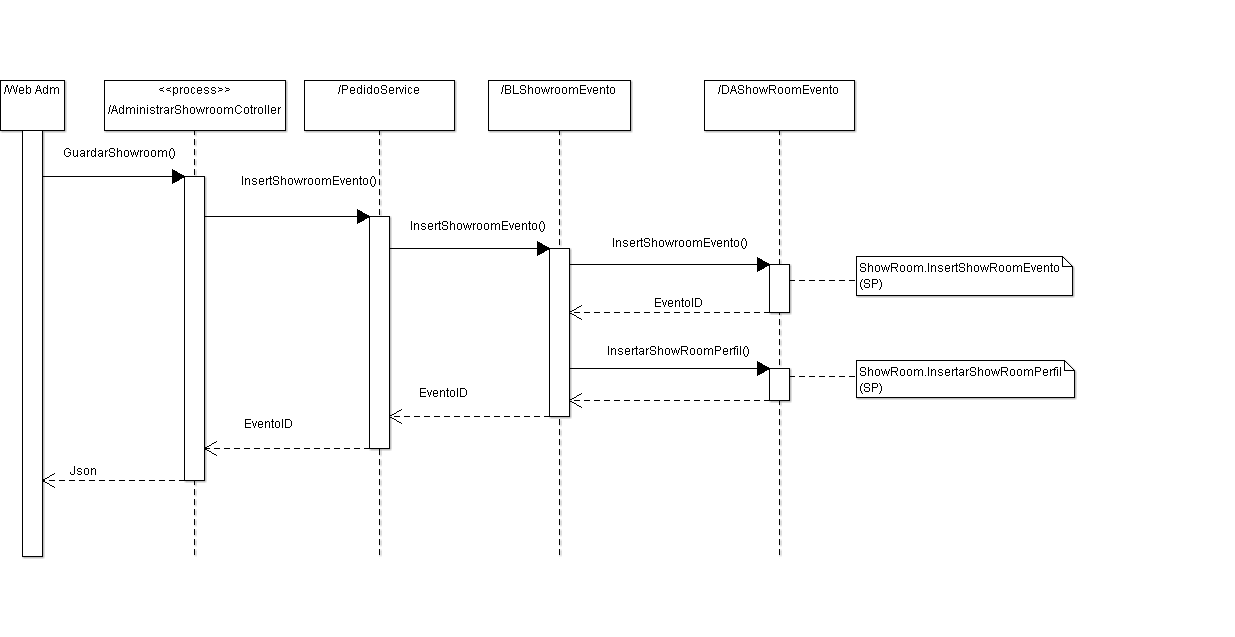
\includegraphics[width=1.5\textwidth]{imgs/Eventos/NuevoEvento.png}
\caption{Diagrama de secuencia Creación de Evento}
\end{figure}
\end{landscape} 

\lstinputlisting[style=Sql]{InsertShowRoomEvento.sql}
\lstinputlisting[style=Sql]{InsertarShowRoomPerfil.sql}



\newpage
\subsubsection{Editar Evento}

\begin{figure}[h]
\centering
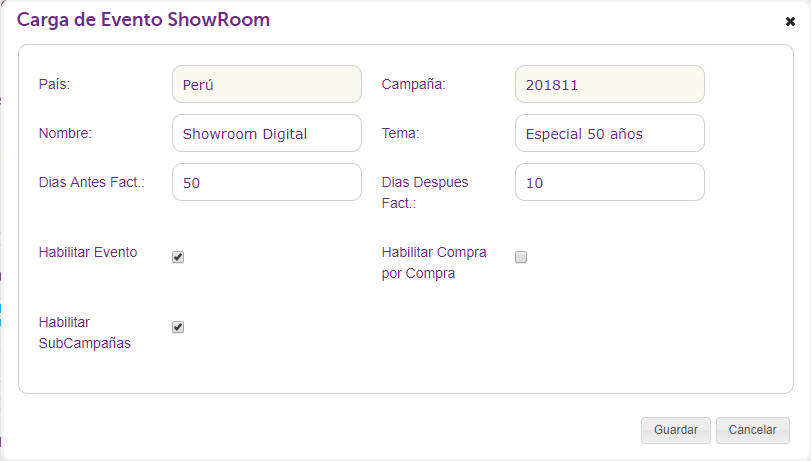
\includegraphics[width=1.0\textwidth]{imgs/Eventos/FormularioEditarEvento.png}
\caption{Formulario para administrar eventos}
\end{figure}

\begin{landscape}
\begin{figure}[!h]
\centering
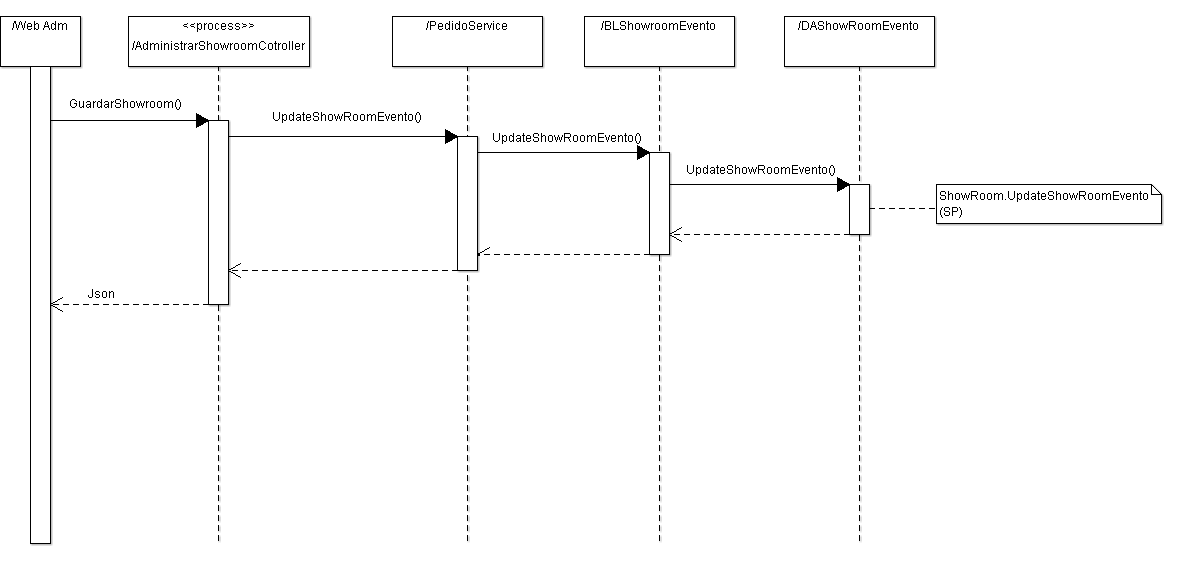
\includegraphics[width=1.5\textwidth]{imgs/Eventos/EditarEvento.png}
\caption{Diagrama de secuencia Edición de Evento}
\end{figure}
\end{landscape} 

\lstinputlisting[style=Sql]{UpdateShowRoomEvento.sql}


\newpage
\subsubsection{Deshabilitar Evento}

\begin{figure}[h]
\centering
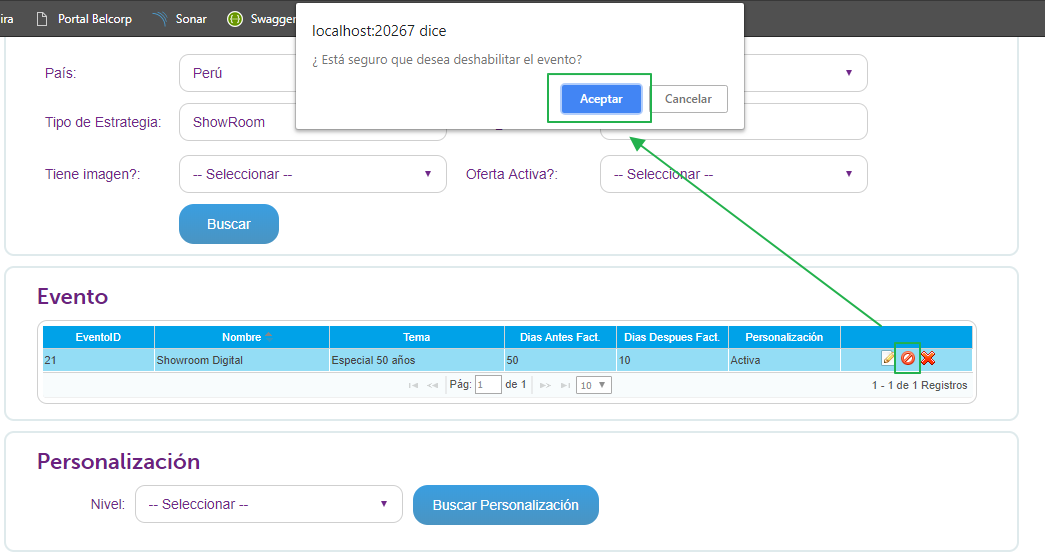
\includegraphics[width=1.0\textwidth]{imgs/Eventos/FormularioDeshabilitarEvento.png}
\caption{Formulario para deshabilitar eventos}
\end{figure}


\begin{landscape}
\begin{figure}[!h]
\centering
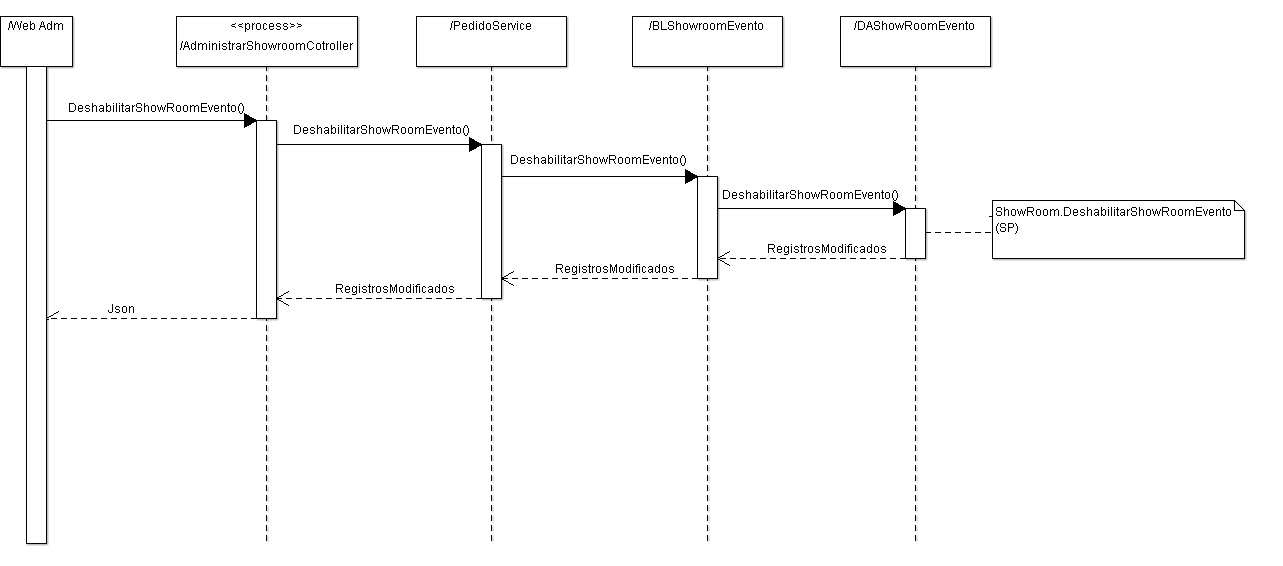
\includegraphics[width=1.5\textwidth]{imgs/Eventos/DeshabilitarEvento.png}
\caption{Diagrama de secuencia Inactivación de Evento}
\end{figure}
\end{landscape} 

\lstinputlisting[style=Sql]{DeshabilitarShowRoomEvento.sql}



\newpage
\subsubsection{Eliminar Evento}

\begin{figure}[h]
\centering
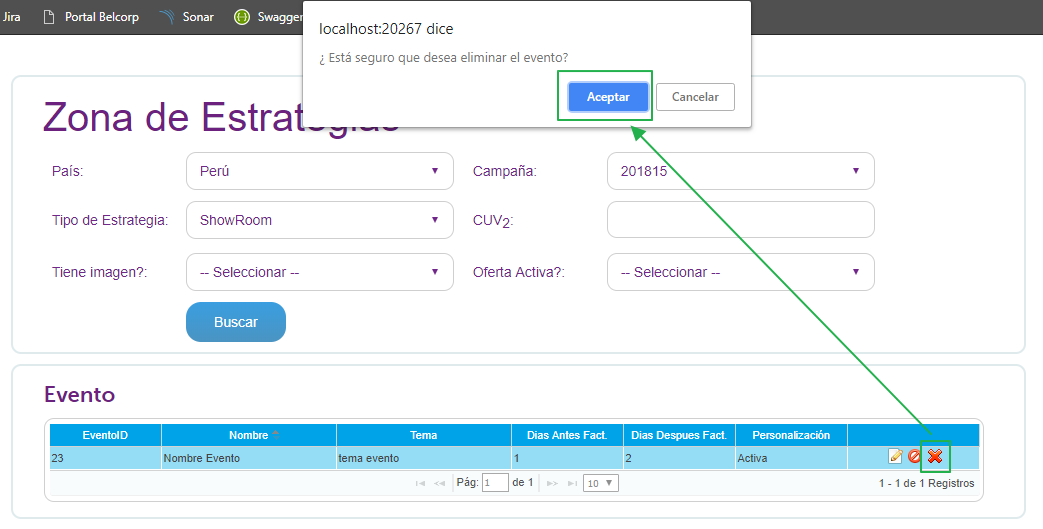
\includegraphics[width=1.0\textwidth]{imgs/Eventos/FormularioEliminarEvento.png}
\caption{Formulario para eliminar eventos}
\end{figure}


\begin{landscape}
\begin{figure}[!h]
\centering
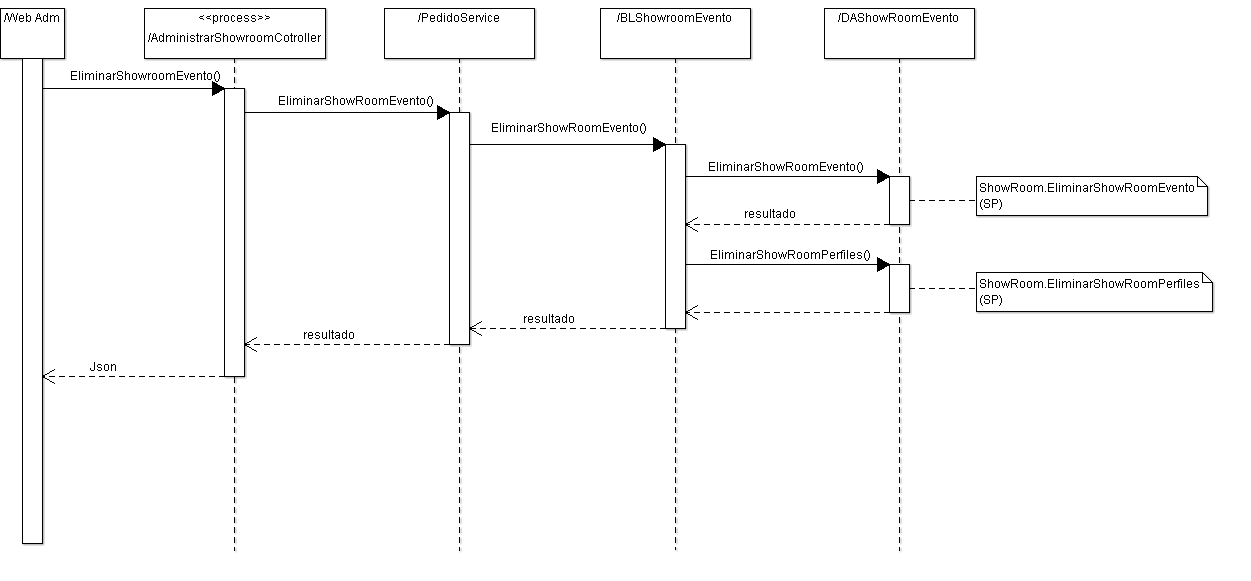
\includegraphics[width=1.5\textwidth]{imgs/Eventos/EliminarEvento.png}
\caption{Diagrama de secuencia Eliminación de Evento}
\end{figure}
\end{landscape} 

\lstinputlisting[style=Sql]{EliminarShowRoomEvento.sql}
\lstinputlisting[style=Sql]{EliminarShowRoomPerfiles.sql}


%%%----------%%%----------PERSONALIZACIÓN----------%%%----------%%%

\newpage
\subsection{Gestión de personalización}

\subsubsection{Modelo relacional}
\begin{figure}[h]
\centering
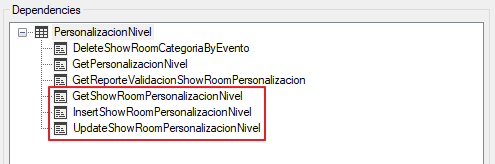
\includegraphics[width=1.0\textwidth]{imgs/Personalizacion/SPsAdmPersonalizacionNivel.png}
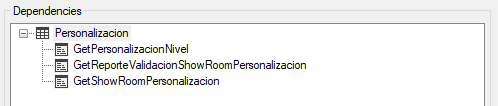
\includegraphics[width=1.0\textwidth]{imgs/Personalizacion/SPsAdmPersonalizacion.png}
\caption{Procedimientos almacenados administrador de contenido}
\end{figure}

\begin{figure}[!h]
\centering
\includegraphics[width=1.0\textwidth]{imgs/Personalizacion/Tablas.png}
\caption{Tablas para Personalizaciones}
\end{figure}

\begin{figure}[!h]
\centering
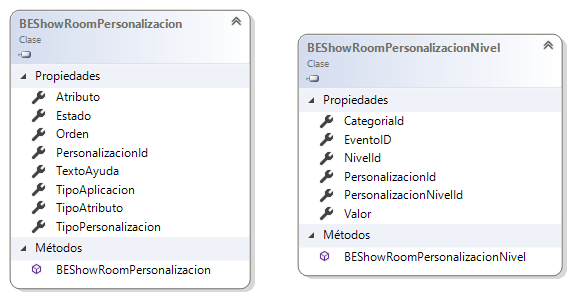
\includegraphics[width=1.0\textwidth]{imgs/Personalizacion/EntidadPersonalizacion.png}
\caption{Entidades Personalización}
\end{figure}

\newpage
\subsubsection{Buscar Personalización}

\begin{figure}[h]
\centering
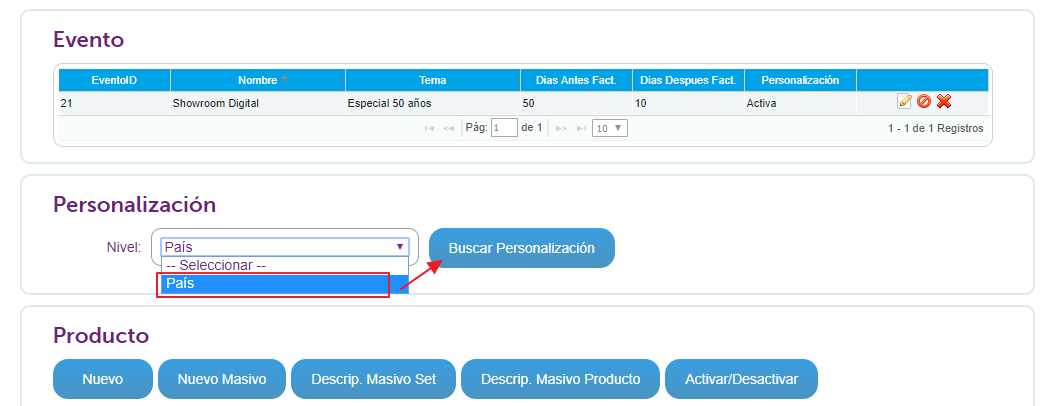
\includegraphics[width=1.0\textwidth]{imgs/Personalizacion/FormularioBuscarPersonalizacion.png}
\caption{Formulario para búsqueda de personalización}
\end{figure}

\begin{landscape}
\begin{figure}[!h]
\centering
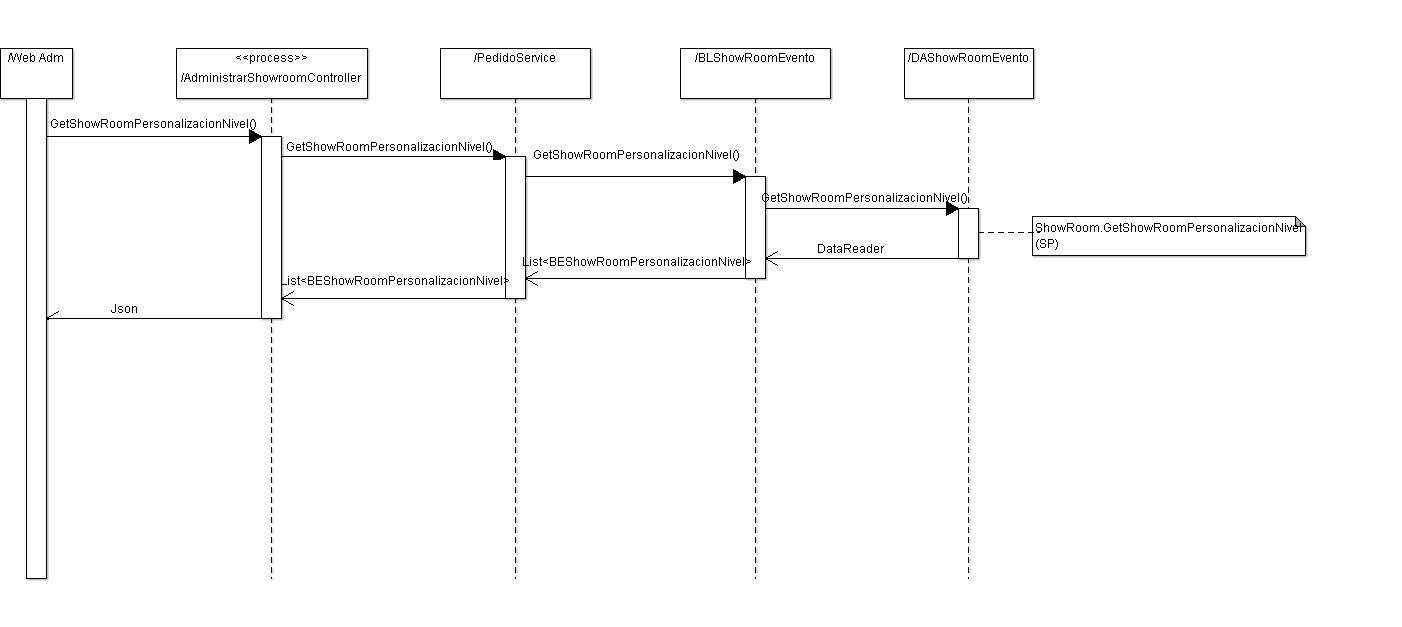
\includegraphics[width=1.5\textwidth]{imgs/Personalizacion/BuscarPersonalizacion.png}
\caption{Diagrama de secuencia Búsqueda de Personalización}
\end{figure}
\end{landscape} 

\lstinputlisting[style=Sql]{GetShowRoomPersonalizacionNivel.sql}



\newpage
\subsubsection{Editar Personalización}

\begin{figure}[h!]
\centering
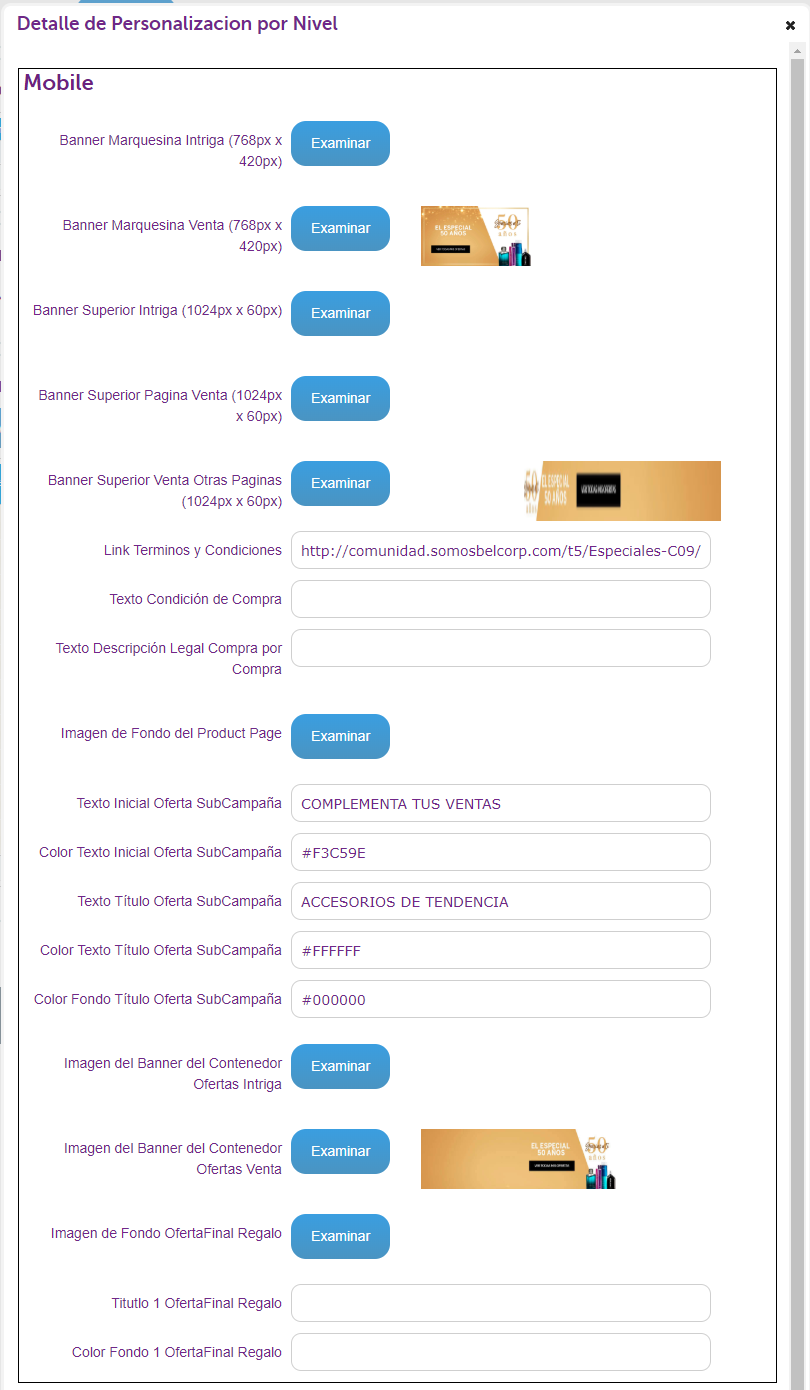
\includegraphics[width=0.7\textwidth]{imgs/Personalizacion/FormularioEditarPersonalizacionMobile.png}
\caption{Formulario para edición de personalización mobile}
\end{figure}

\begin{figure}[h]
\centering
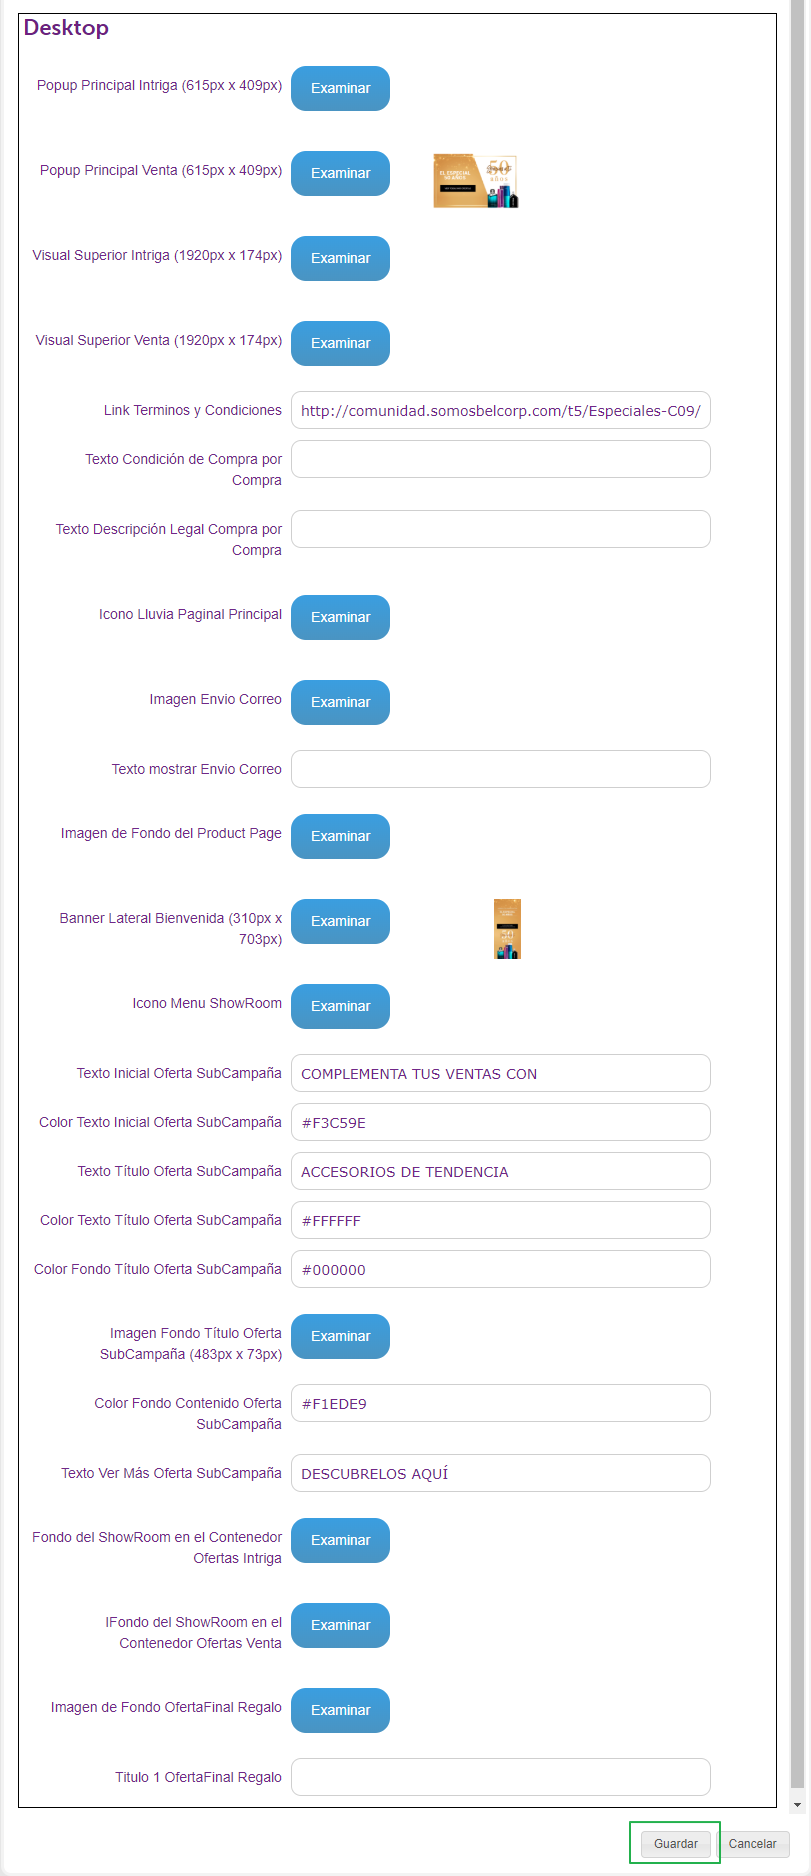
\includegraphics[width=0.65\textwidth]{imgs/Personalizacion/FormularioEditarPersonalizacionDesktop.png}
\caption{Formulario para edición de personalización desktop}
\end{figure}

\begin{landscape}
\begin{figure}[!h]
\centering
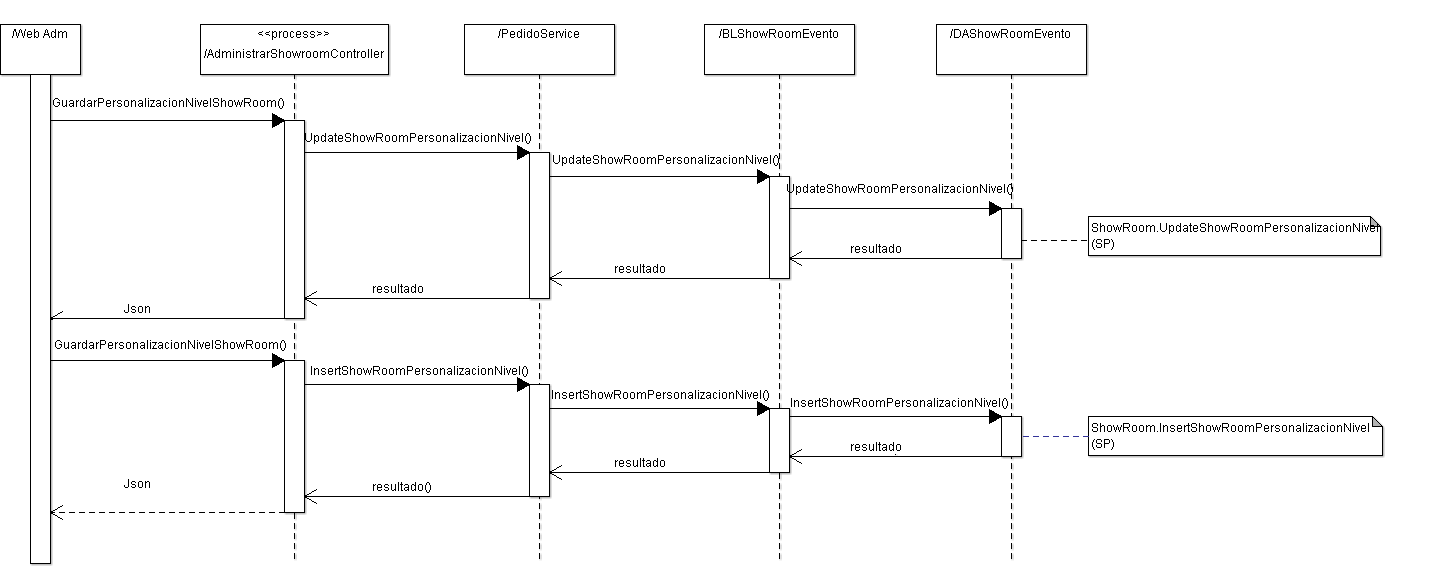
\includegraphics[width=1.5\textwidth]{imgs/Personalizacion/GuardarPersonalizacion.png}
\caption{Diagrama de secuencia Edición de Personalización}
\end{figure}
\end{landscape} 

\lstinputlisting[style=Sql]{UpdateShowRoomPersonalizacionNivel.sql}
\lstinputlisting[style=Sql]{InsertShowRoomPersonalizacionNivel.sql}


%%%----------%%%----------PRODUCTOS----------%%%----------%%%

\newpage
\subsection{Gestión de productos}

\begin{figure}[h]
\centering
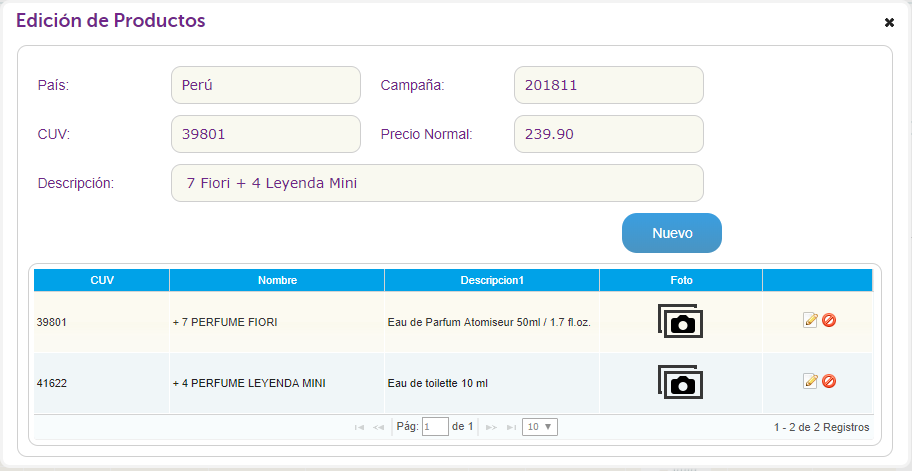
\includegraphics[width=1.0\textwidth]{imgs/Producto/FormularioGestionProductos.png}
\caption{Formulario para administrar productos}
\end{figure}

\newpage
\begin{figure}[h!]
\centering
\includegraphics[width=0.8\textwidth]{imgs/Producto/Tablas.png}
\caption{Tablas Estrategia Producto}
\end{figure}

\newpage
\begin{figure}[h!]
\centering
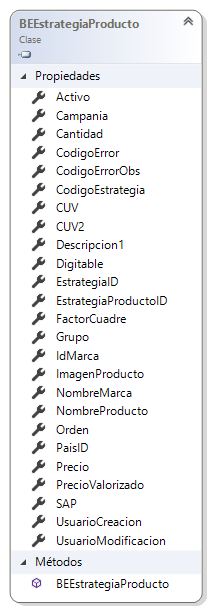
\includegraphics[width=0.5\textwidth]{imgs/Producto/EntidadProducto.png}
\caption{Entidad Estrategia Producto}
\end{figure}

\newpage
\subsubsection{Consultar Producto}

\begin{figure}[h!]
\centering
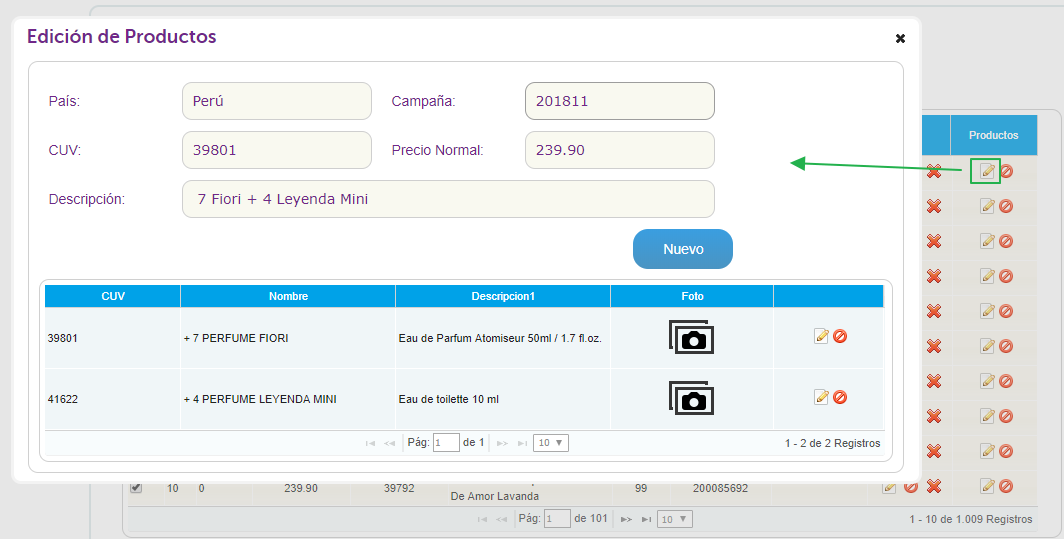
\includegraphics[width=1.0\textwidth]{imgs/Producto/FormularioConsultarProducto.png}
\caption{Consultar productos de una estrategia}
\end{figure}

\begin{landscape}
\begin{figure}[!h]
\centering
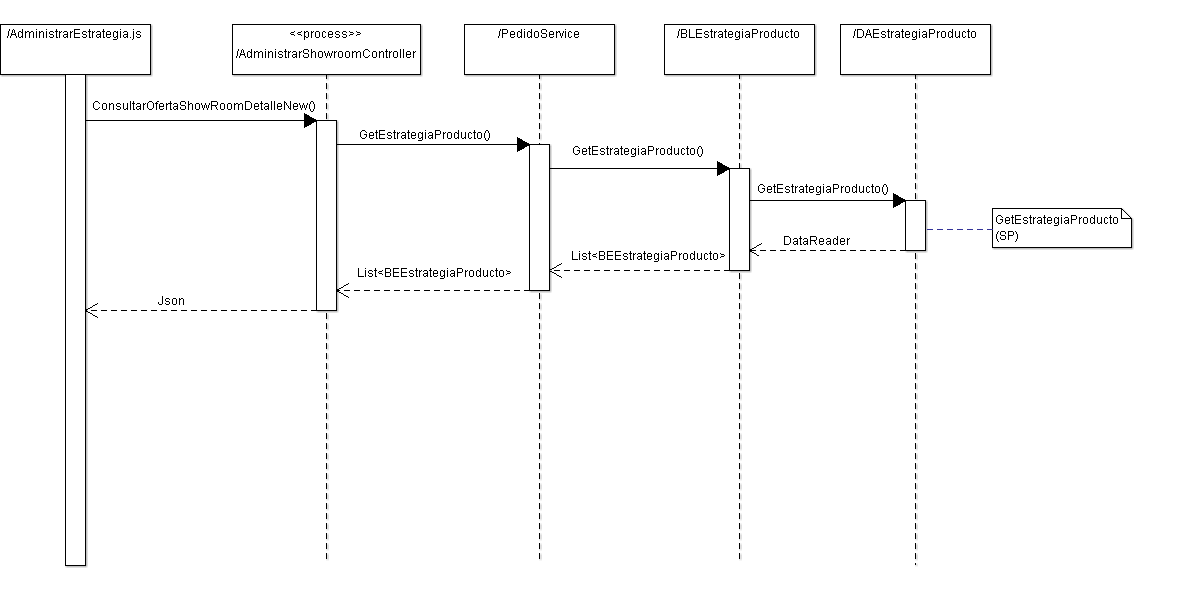
\includegraphics[width=1.5\textwidth]{imgs/Producto/ConsultarProducto.png}
\caption{Diagrama de secuencia Contulta de producto}
\end{figure}
\end{landscape} 

\lstinputlisting[style=Sql]{GetEstrategiaProducto.sql}

\newpage
\subsubsection{Crear Producto}

\begin{figure}[h]
\centering
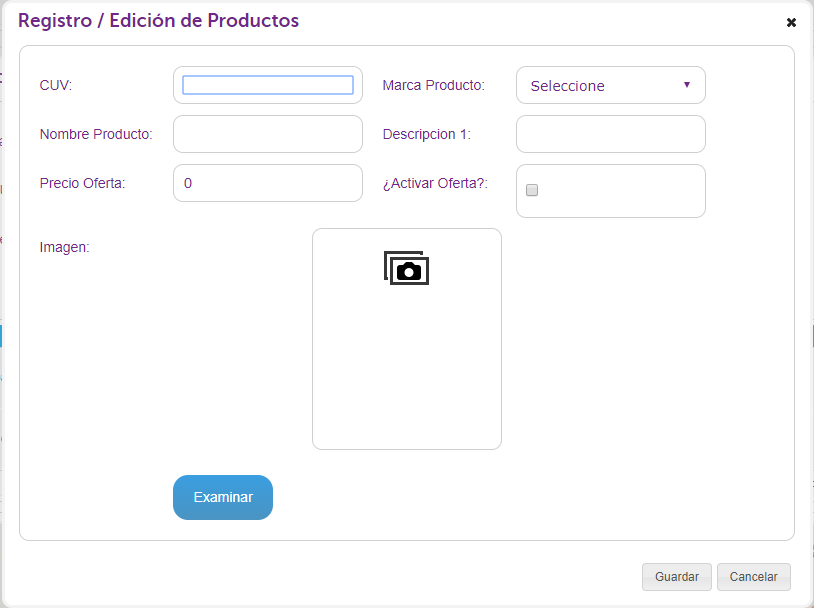
\includegraphics[width=1.0\textwidth]{imgs/Producto/FormularioNuevoProducto.png}
\caption{Formulario para nuevo producto}
\end{figure}

\begin{landscape}
\begin{figure}[!h]
\centering
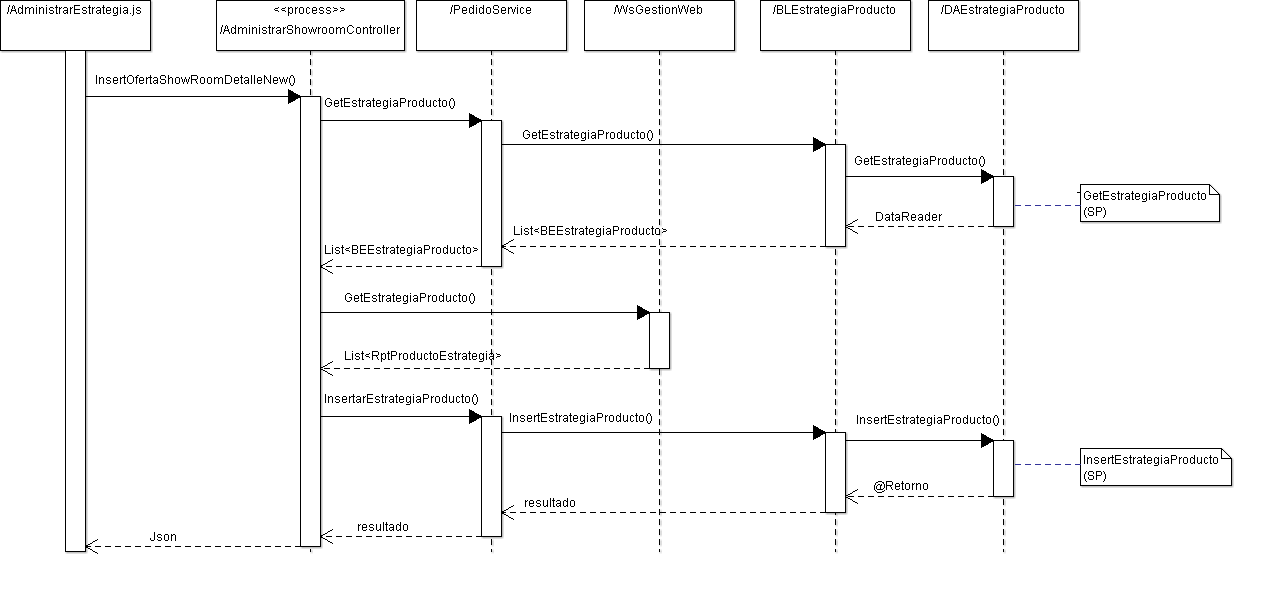
\includegraphics[width=1.5\textwidth]{imgs/Producto/InsertarProducto.png}
\caption{Diagrama de secuencia Insertar producto}
\end{figure}
\end{landscape} 

\lstinputlisting[style=Sql]{InsertEstrategiaProducto.sql}



\newpage
\subsubsection{Editar Producto}

\begin{figure}[h]
\centering
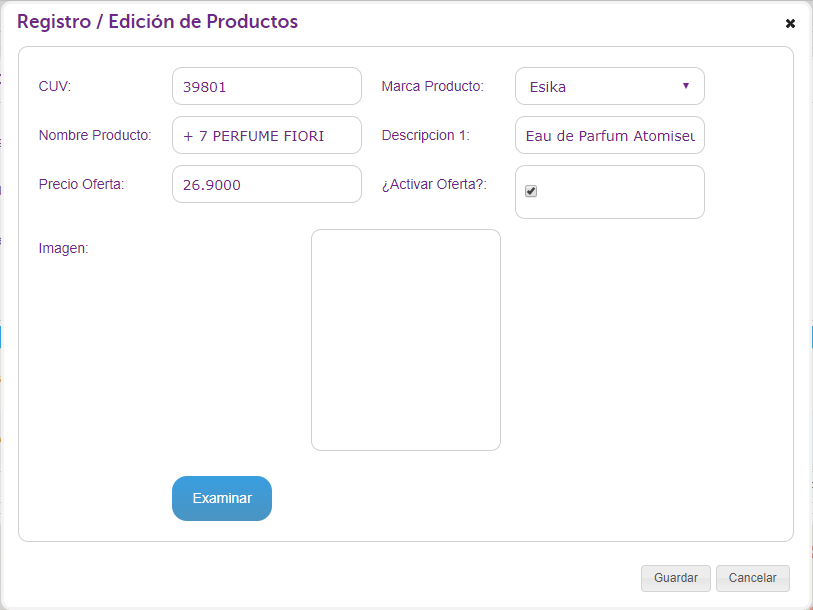
\includegraphics[width=1.0\textwidth]{imgs/Producto/FormularioEditarProducto.png}
\caption{Formulario de edición de productos}
\end{figure}

\begin{landscape}
\begin{figure}[!h]
\centering
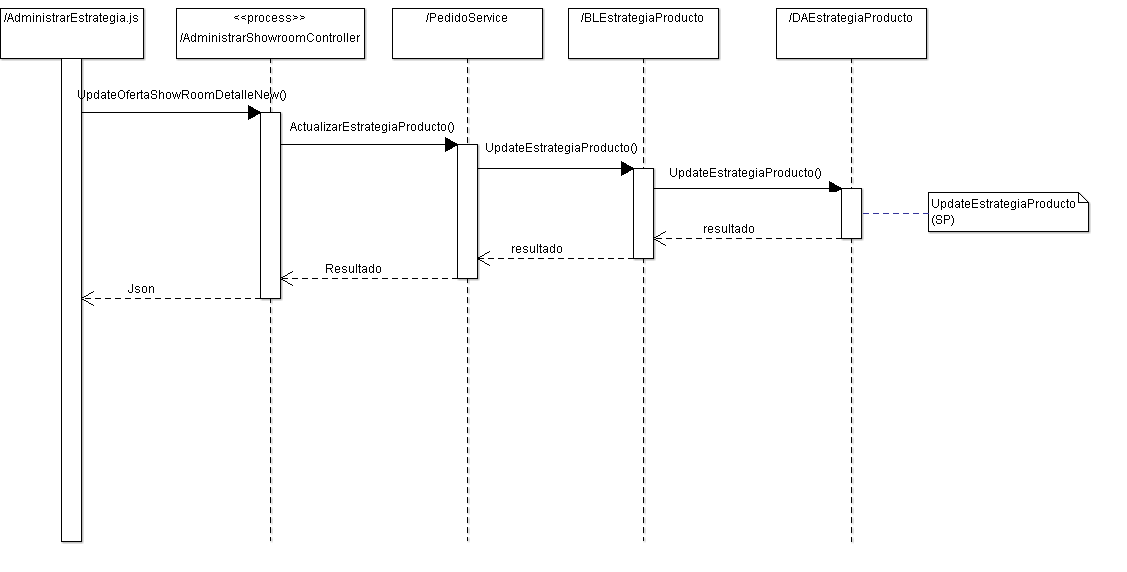
\includegraphics[width=1.5\textwidth]{imgs/Producto/EditarProducto.png}
\caption{Diagrama de secuencia Editar producto}
\end{figure}
\end{landscape} 

\lstinputlisting[style=Sql]{UpdateEstrategiaProducto.sql}



\newpage
\subsubsection{Deshabilitar Producto}
\begin{figure}[h]
\centering
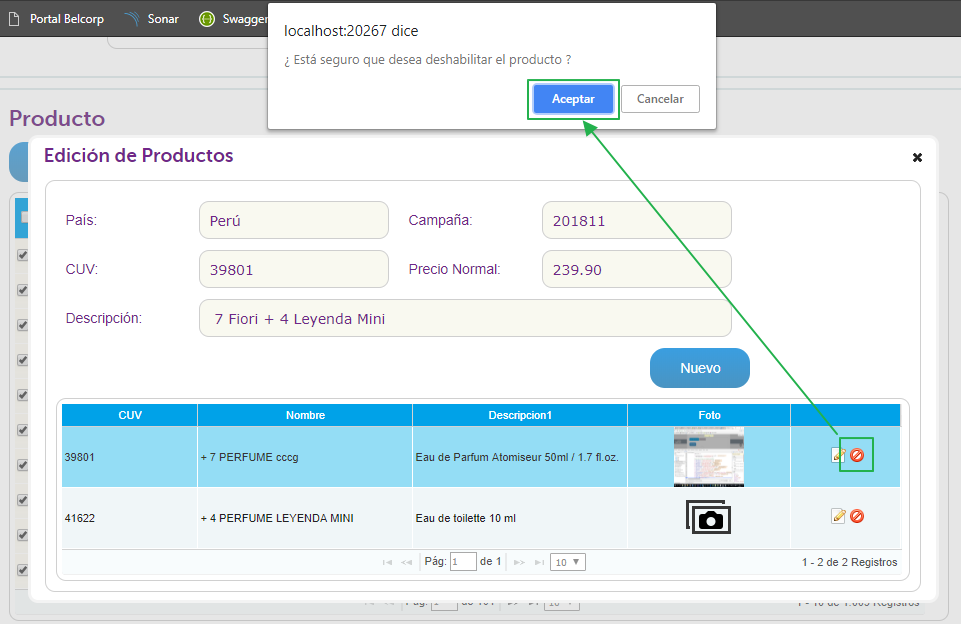
\includegraphics[width=1.0\textwidth]{imgs/Producto/FormularioDeshabilitarProducto.png}
\caption{Formulario para Deshabilitar productos}
\end{figure}

\begin{landscape}
\begin{figure}[!h]
\centering
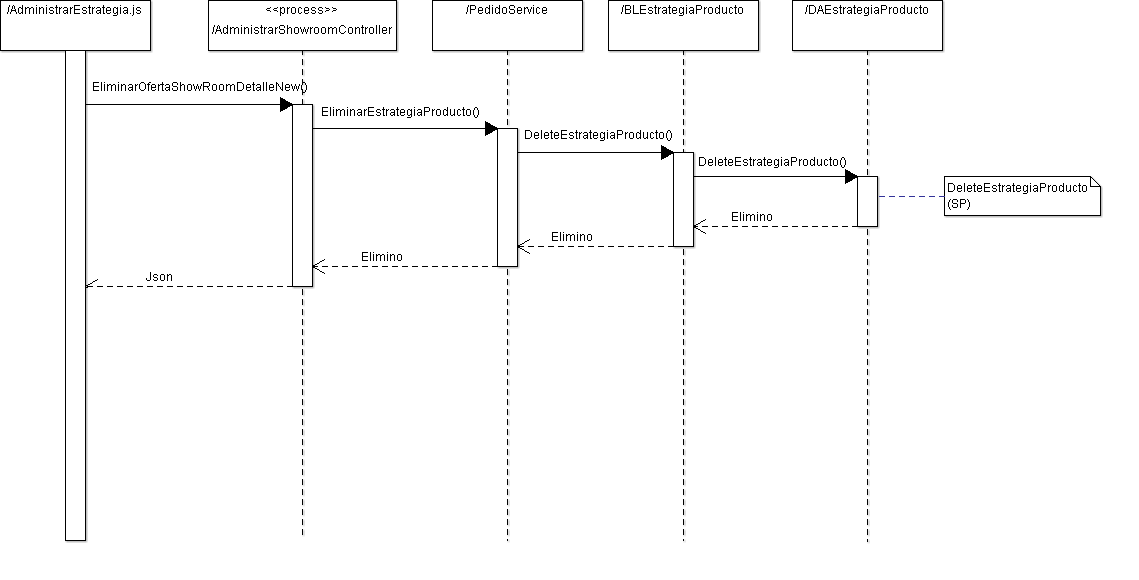
\includegraphics[width=1.5\textwidth]{imgs/Producto/EliminarProducto.png}
\caption{Diagrama de secuencia Deshabilitar Producto}
\end{figure}
\end{landscape} 

\lstinputlisting[style=Sql]{DeleteEstrategiaProducto.sql}


\newpage
\subsubsection{Deshabilitar Productos por Set}
\begin{figure}[h]
\centering
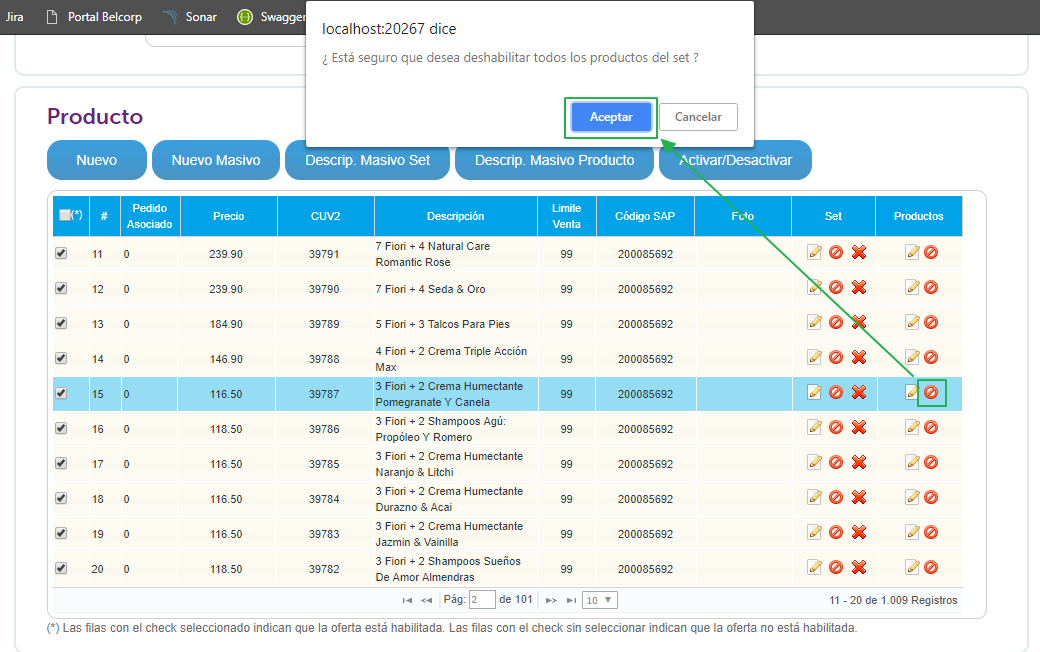
\includegraphics[width=1.0\textwidth]{imgs/Producto/FormularioDeshabilitarTodosProducto.png}
\caption{Formulario para Deshabilitar productos por set}
\end{figure}


\begin{landscape}
\begin{figure}[!h]
\centering
\includegraphics[width=1.5\textwidth]{imgs/Producto/EliminarTodo.png}
\caption{Diagrama de secuencia Deshabilitar productos por set}
\end{figure}
\end{landscape} 

\lstinputlisting[style=Sql]{DeleteEstrategiaProductoAll.sql}

\newpage
\subsubsection{Actualizar Descripción Masiva Producto}

\begin{figure}[h]
\centering
\includegraphics[width=1.0\textwidth]{imgs/Producto/FormularioActualizarDescripcionMasivaProducto.png}
\caption{Formulario para Actualizar Descripción Masiva Producto}
\end{figure}

\newpage
\begin{landscape}
\begin{figure}[!h]
\centering
\includegraphics[width=1.5\textwidth]{imgs/Producto/InsertarMasivoProducto.png}
\caption{Diagrama de secuencia Actualizar Descripción Masiva Producto}
\end{figure}
\end{landscape} 

\lstinputlisting[style=Sql]{InsertarProductoShowroomMasiva.sql}

\newpage
\section{Portal Somos Belcorp}
\subsection{Versión Web}
\subsection{Versión Mobil}


\end{document}